\section{Spezifikation der Inventursoftware} \label{software}

Um die Bilddaten der Drohne für eine Inventur zu verarbeiten, soll die Drohne von einer Client-Anwendung angesprochen werden. Der Server, der als Client agiert und im \textit{Flask} Framework für Python zu schreiben ist, verbindet sich zur Drohne und sendet die Flugsignale als Fluganweisungen zur Drohne. Da die Drohne keinerlei Sensoren zur Detektion möglicher Hindernisse enthält und es zudem nicht das Ziel ist, die Drohne automatisiert fliegen zu lassen, wird die Flugroute statisch als Flugsequenz festgelegt. 

Auf dem Server ist zudem das \textit{Deep Learning} Modell zur Inferenz integriert. Der Server inferiert die von der Drohne empfangenen Video-Stream-Frames mit dem Modell, zählt die detektierten Objekte und gibt die Bilddaten mit den eingezeichneten Bounding Boxen anschließend per Livestream an eine Webapplikation zur Visualisierung weiter. Eine \textit{REST} Schnittstelle gibt Aussage über die Bestandsdaten des Warenhauses.

\begin{figure}[ht]
	\begin{center}
		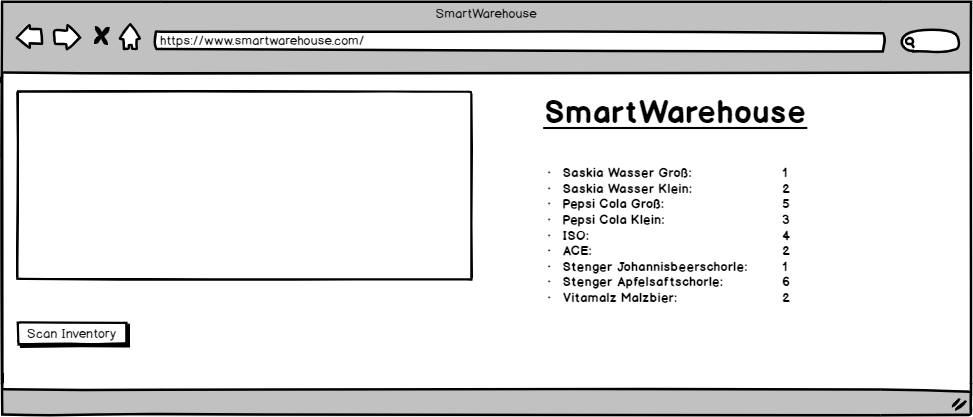
\includegraphics[width=15cm]{Bilder/UI.png} 
		\caption[SmartWarehouse User Interface]{SmartWarehouse User Interface}
		\label{ui}
	\end{center}
\end{figure}

Die Client-Anwendung zeigt das Live-Drohnenbild mit den eingezeichneten, erkannten Objekten. Zudem wird die Anzahl an erkannten Objekten der spezifischen Klassen rechts daneben dargestellt. 
